% LaTeX Template for short student reports.
% Citations should be in bibtex format and go in references.bib
\documentclass[a4paper, 11pt]{article}
\usepackage[top=3cm, bottom=3cm, left = 2cm, right = 2cm]{geometry}
\geometry{a4paper}
\usepackage[utf8]{inputenc}
\usepackage{textcomp}
\usepackage{graphicx}
\usepackage{amsmath,amssymb}
\usepackage{bm}
\usepackage[bookmarks,colorlinks,breaklinks]{hyperref}
\usepackage{algpseudocode}
\usepackage{algorithm}
\hypersetup{linkcolor=black,citecolor=black,filecolor=black,urlcolor=black}
% % black links, for printed output
\usepackage{minted}
\usepackage{memhfixc}
\usepackage{pdfsync}
\usepackage{fancyhdr}
\pagestyle{fancy}

\title{Gradient Boosting Trees}
\author{Nimrod Ohayon Rozanes}
%\date{}

\begin{document}
\maketitle
\break
\tableofcontents
\break
\section{Introduction}

This report details the design, implementation, and testing of
gradient boosting trees. In the first section, the theory of base desicion
trees and gradient trees are detailed, then a description and
derivation of the XGBoost algorithm is given; in this section, the
performance and computational cost will also be analyzed. Afterwards, the
implementation and library design of the the methods is provided,
with particularly noteworthy code exerpts highlighted. Then, the
trees and ensamble methods are tested against multiple data sets,
three natural and two synthetic, which illustrate the trade offs of
each algorithm. In the conclusion, the requirements for this report
are reviewed.

\section{Description and Analysis}
\subsection{Background}

A descision trees is a non-parametric, supervized model which can be
used both as a regressor and as a classifier. In either case, the
model does not make any assumptions about the basic shape of the
data, partially because of this, and because of the fact that it is a
usually very natural thing to think about data being related to it's
label through the recursive relationship which a tree captures well,
descision trees are a very popular tool. Descision tree's are also
able to handle very high dimensional data sets and multiclass
problems very well which often make them a more natural model when
compared to an algorithm like k-NN, which will struggle in higher
dimensions, or the logistic regression, which has to be retrofitted
to handle multiclass problems.

Built on top of the basic desicion tree are a variety of techniques
called ensamble learning methods. Each one addresses a particular
issue that an analyst might face with a particular data set by
combining multiple trees in some fashion. A short description of the
two main families of methods follows:
\begin{itemize}
  \item Random forest methods
    address the high variance of the base tree (which is discussed in
    detail in the following section) by averaging the predictions of
    multiple trees, each trained on a randomized dataset, using a random
    subset of features.
  \item Boosting methods train trees addatively and sequentially. By
    adding together the predictions of multiple trees which are each
    trained based on the results of the last, boosting methods
    address data which is difficult to describe with a tree of
    reasonable depth. There are a couple of variants of boosting methods
\end{itemize}

Boosting and bagging remedy two different usually mutually
exclusive issues that can arise while modeling data. However, they are
sometimes combined, usually through boosting each tree of the random
forest, when the random forest does not achieve sufficient accuracy
in its predictions.

Gradient boosting generalizes the boosting procedure to use an
arbitrary gradient, which can be supplied by the user. XGBoost is an
algorithm which improves boosted trees in basically all accounts, and
its core is based on utilizing second order information about the
loss to improve iterations.

\subsection{Descision Trees}

\subsubsection{Algorithm}

Given data of the form $(x^i, y^i)$ where $x^i$ is a vector of either
categorical or continuous variables, and $y^i$ is the variable we
would like to inference, categorical in the classification task and
continuous in the regression task, construct an appropriate loss
function $L(\hat y, y)$ which evaluates the appropriateness of a
prediction $\hat y$ to the actual value $y$. The symbols used are:

\begin{center}
  \begin{tabular}{ll}
    $\mathcal{D}$               & training dataset $\{(x^i, y^i)\}$ \\
    $d_{\max}$                  & maximum allowed depth of the tree \\
    $n_{\min}$                  & minimum samples required to split a node \\
    $L(c, y)$                   & loss between prediction $c$ and label $y$ \\
    $\mathcal{L}(\mathcal{D})$  & aggregate loss (impurity) over a
    set $\mathcal{D}$ \\
    $j,\; t$                    & candidate feature index and split threshold \\
    $j^*,\; t^*$                & optimal feature and threshold at a node \\
    $\mathcal{D}_L,\;\mathcal{D}_R$ & left and right partitions
    induced by $(j^*, t^*)$ \\
  \end{tabular}
\end{center}

We now construct the tree in the following manner:
% \usepackage{algorithm,algorithmicx,algpseudocode}
\begin{algorithm}
  \floatname{algorithm}{Algorithm}
  \caption{Descision Tree}\label{alg:}
  \begin{algorithmic}[1]
    \Procedure{BuildTree}{$\mathcal{D},\, d_{\max}$}
    \If{$d_{\max} = 0$ \textbf{or} $|\mathcal{D}| < n_{\min}$
    \textbf{or} all $y^i$ identical}
    \State \Return $\mathrm{Leaf}\!\left(\hat{y} =
    \displaystyle\arg\min_{c}\sum_{i \in \mathcal{D}} L(c,\, y^i)\right)$
    \EndIf
    \State Find best split:
    \State \quad $(j^*, t^*) \gets \displaystyle\arg\min_{j,\,t}\;
    \frac{|\mathcal{D}_L|}{|\mathcal{D}|}\,\mathcal{L}(\mathcal{D}_L)
    + \frac{|\mathcal{D}_R|}{|\mathcal{D}|}\,\mathcal{L}(\mathcal{D}_R)$
    \State \quad where $\mathcal{D}_L = \{(x^i, y^i) \in \mathcal{D}
    : x^i_{j} \leq t\}$,\; $\mathcal{D}_R = \mathcal{D} \setminus \mathcal{D}_L$
    \State $\mathrm{left}  \gets$
    \Call{BuildTree}{$\mathcal{D}_{L},\; d_{\max} - 1$}
    \State $\mathrm{right} \gets$
    \Call{BuildTree}{$\mathcal{D}_{R},\; d_{\max} - 1$}
    \State \Return $\mathrm{Node}(j^*,\; t^*,\; \mathrm{left},\;
    \mathrm{right})$
    \EndProcedure
  \end{algorithmic}
\end{algorithm}

\subsubsection{Training}

Unsurprisingly, the algorithm is best described recursively. In
words, at each level of the tree, we look for the best possible split
of the data that this node sees. We find this best split by looking
through every possible split point, which is the middle between every
point in every feature of $x$, then evaluating the total loss on
either the left or the right side if we were to make this split, once
we find the point which minimizes the loss over all possible splits,
we choose that as the split at this node, then run the procedure
again, only this time another level down, and with the dataset
partitioned between left and right. There are a couple of important
caveats, namely, it's often more natural for the split finder to seek
maximizing some gain function rather than minimize a loss function;
in the classification task, it is common to state the goal as
maximizing the information gain at each split; since the parent
entropy is fixed at each node, this is equivalent to minimizing
the weighted average entropy of the two child partitions.

\subsubsection{Prediction}

Given a data point $x$, prediction proceeds by traversing the tree
from root to leaf: at each internal node with stored feature index
$j^*$ and threshold $t^*$, route $x$ to the left child if
$x_{j^*} \leq t^*$ and to the right child otherwise. At the leaf,
return the stored value $\hat{y}$, which is the mean of the training
samples that fell there in the regression case, or the majority class
(or full class-probability vector) in the classification case. Each
step descends exactly one level, so prediction costs $O(d_{\max})$
comparisons.

\subsubsection{Complexity}

For training, finding the best split at a single node with $n$ samples
and $f$ features requires evaluating each of the $n - 1$ candidate
thresholds per feature. If each feature's values are pre-sorted, the
impurity of each candidate split can be updated incrementally in
$O(1)$, giving $O(fn)$ work per node. Because the data is partitioned
disjointly across all nodes at a given depth, the total work per depth
level is also $O(fn)$, and summing over $d_{\max}$ levels gives
$O(fn \, d_{\max})$. Pre-sorting all features once costs
$O(fn \log n)$, so the total training complexity is
$O\!\left(fn(d_{\max} + \log n)\right)$.
This can become expensive for large $n$ or $f$, and approximate
split-finding methods (e.g.\ histogram binning) are common in
production implementations.

\subsubsection{Overfitting and Regularization}

The essential feature of a tree is that, given an unlimited
$d_{\text{max}}$ a descision tree will always
overfit. This is because if there is no limit on the number of leaves
that the tree can create, the tree will happily split the data down
into individual data points, perfectly classifying each data point in
the training set while likely performing terribly on the test set. As
such, it is common to prune trees after they are fit, or deciding on
a minimum loss decrease that a split must exhibit before a split is
added to the tree. A more extensive discussion of pruning and
regularization will take place when discussing XGBoost.
In this way,
the depth of a tree decides the model complexity: a deeper tree will
tend have very high variance and a low bias, and very shallow tree
will have lower variance but higher bias, the exact optimal depth is
dataset dependent, and generally not easy to find.
Trees are
also, in general, not optimal since the split finding approach is
greedy, the tree chooses the best split in the local context, not
considering any future splits.

\subsection{Gradient Boosting Trees}

\subsubsection{Algorithm}

Given a differentiable loss function $L(\hat{y}, y)$ and a dataset
$\mathcal{D} = \{(x^i, y^i)\}_{i=1}^{n}$, gradient boosting builds
an additive model $F_M(x) = \sum_{m=0}^{M} \eta \, h_m(x)$, where
each $h_m$ is a shallow tree and $\eta \in (0,1]$ is a learning rate.

\begin{algorithm}
  \floatname{algorithm}{Algorithm}
  \caption{Gradient Boosting}\label{alg:gb}
  \begin{algorithmic}[1]
    \State Initialize $F_0(x) = \displaystyle\arg\min_{c}
    \sum_{i=1}^{n} L(c,\, y^i)$
    \For{$m = 1$ \textbf{to} $M$}
    \State Compute pseudo-residuals:
    $r^i_m = -\dfrac{\partial L(F_{m-1}(x^i),\, y^i)}
    {\partial F_{m-1}(x^i)}$
    \quad for all $i$
    \State Fit a regression tree $h_m$ to
    $\{(x^i,\, r^i_m)\}_{i=1}^{n}$
    \State For each leaf $\ell$ of $h_m$, set optimal leaf value:
    $\gamma_\ell = \displaystyle\arg\min_{\gamma}
    \sum_{i \in \ell} L\!\left(F_{m-1}(x^i) + \gamma,\; y^i\right)$
    \State Update: $F_m(x) = F_{m-1}(x) + \eta \, h_m(x)$
    \EndFor
    \State \Return $F_M$
  \end{algorithmic}
\end{algorithm}

\subsubsection{Pseudo-Residuals and Function-Space Gradient Descent}

We initialize the simplest possible prediction to the data set, which
ever constant minimizes the loss over the whole data set. From there
we begin to instead learn the negative gradient of the loss function
with respect to the current predictions. Then the leaves of the tree
which we fitted to the negative gradient are set to the be the value
which once added to the last prediction, minimizes the loss of the last tree.
The key insight is that fitting each new tree to the negative gradient
of the loss is a steepest-descent step in function space.

In a more classical set up, gradient descent would be applied to the
parameters of the model; this approach is difficult to apply to a
tree due to the number of parameters being often variable. Instead,
in the graident boosting model, we treat the model $F$ itself as the
subject of gradient descent optimization. We are generally not able
to move freely in function space, that is, it is difficult to
describe a direction in function space, as such we approximate the
direction we'd like to move in through a tree. In principle, we can
use other models in place of a tree when approximating the pseudo-residuals.

In the case of MSE loss, the gradient collapses neatly into the
literal residuals of the last model. With
$L(\hat{y}, y) = \tfrac{1}{2}(\hat{y} - y)^2$,
\[
  r^i_m
  = -\frac{\partial L(F_{m-1}(x^i),\, y^i)}{\partial F_{m-1}(x^i)}
  = -\frac{\partial}{\partial F_{m-1}(x^i)}
  \tfrac{1}{2}\!\left(F_{m-1}(x^i) - y^i\right)^2
  = -\!\left(F_{m-1}(x^i) - y^i\right)
  = y^i - F_{m-1}(x^i).
\]
For other losses the negative
gradient plays the same corrective role but is not a simple
difference.

\subsubsection{Complexity}

Each iteration of gradient boosting fits one regression tree to the
pseudo-residuals, which costs $O\!\left(fn(d_{\max} + \log n)\right)$
as derived in the decision tree section. Over $M$ iterations the
total training cost is therefore
\[
  O\!\left(M \cdot fn(d_{\max} + \log n)\right).
\]
In addition, computing the pseudo-residuals requires one forward pass
through the current ensemble per sample, which at iteration $m$ costs
$O(m \cdot d_{\max})$ per sample and $O(m \cdot n \cdot d_{\max})$
over the dataset; summed over all $M$ iterations this contributes
$O(M^2 n d_{\max})$. In practice $d_{\max}$ is small (often 3--6)
and the tree-fitting term dominates, giving an effective cost of
$O(Mfn \log n)$.

A key consequence of the sequential structure is that the $M$ trees
\emph{cannot} be trained in parallel, unlike the trees of a random
forest. Each tree depends on the residuals of the previous ensemble,
so the algorithm is inherently sequential. Parallelism can still be
exploited \emph{within} each tree (e.g.\ parallelising the split
search across features), but the outer loop over boosting rounds is
a serial bottleneck. This is one of the main practical trade-offs
of gradient boosting relative to bagging methods.

\subsubsection{Bias-Variance Trade-off}

As discusses in the descision tree section, a single deep decision
tree has low bias but very high variance: small changes in the
training data can produce drastically different
splits. Gradient boosting addresses this by combining many
\emph{shallow} trees, each of which is a high-bias, low-variance
learner. Each tree corrects the residual error of the ensemble so
far, reducing bias over iterations in a slow and controlled manner ,
while the shallowness of each individual tree keeps the variance of
each correction small.

Depth $d_{\max}$ of each tree plays the same role here as for the base tree:
deeper trees per round lower bias faster but increase variance per
step. In practice $d_{\max} \in \{3,4,5\}$ is a common default that
keeps each tree a weak learner while still capturing low-order
feature interactions.

\subsection{XGBoost}

XGBoost is a bit different from the prior two algorithms because XGBoost is,
in actuality, one specific code base, rather than a generic
algorithm. As an operational description, XGBoost is an off the shelf
package which allows an analyst to churn through a lot of data in a
computationally effecient manner, using domain specific loss
functions. For the purposes of this report, XGBoost's core identity
is captured in the following addendums to the gradient boosting algorithm:

\begin{itemize}
  \item second order information on the gradient of the loss function
    with respect to the regressor is incorporated into the descent algorithm.
  \item L1, L2, and structural normalization is incorporated inline
    to the algorithm, removing the need for tree pruning post facto.
  \item Row subsampling: each boosting round trains on a random
    fraction $p \in (0,1]$ of the dataset rather than the full set,
    introducing stochasticity that reduces overfitting and lowers the
    per-iteration cost to $O(pfn(d_{\max} + \log(pn)))$.
  \item Column subsampling: at each split, only a random subset of
    $k \leq f$ features is considered as split candidates, reducing
    the per-split search cost and decorrelating successive trees in
    the same spirit as random forests.
\end{itemize}

Each of these is discussed in its own subsection. It should be noted
that while widespread adoption of the XGBoost code base is, in part, due
to the above improvements, XGBoost also offers incredible performance
improvements and optimizations, and is by design very well fit to run
on distributed systems. This is to say that while the implementation
captures much of the analytical aspects of XGBoost, the larger
XGBoost project is much more than what is described here.

\subsubsection{Second Order Information}

Standard gradient boosting fits each tree to the first-order negative
gradient of the loss. XGBoost instead takes a
second-order Taylor expansion of the loss around the current
prediction $F_{m-1}(x^i)$, using the second order approximation of
the function is typically called Newton's method, for its original
application in finding the roots of an equation:
\[
  L\!\left(F_{m-1}(x^i) + h_m(x^i),\; y^i\right)
  \approx L\!\left(F_{m-1}(x^i),\; y^i\right)
  + g^i\, h_m(x^i)
  + \tfrac{1}{2}\, s^i\, h_m(x^i)^2,
\]
where $g^i = \partial L / \partial F_{m-1}(x^i)$ is the gradient and
$s^i = \partial^2 L / \partial F_{m-1}(x^i)^2$ is the Hessian.
Summing over a leaf $\ell$ and minimising over the leaf output
$\gamma_\ell$ gives the closed-form optimal value
\[
  \gamma_\ell^* = -\frac{\sum_{i \in \ell} g^i}{\sum_{i \in \ell} s^i
  + \lambda},
\]
where $\lambda$ is an L2 regularisation term (see below). The
corresponding gain used to evaluate candidate splits is
\[
  \mathrm{Gain} = \frac{1}{2}\left[
    \frac{G_L^2}{H_L + \lambda}
    + \frac{G_R^2}{H_R + \lambda}
    - \frac{(G_L+G_R)^2}{H_L+H_R+\lambda}
  \right] - \gamma,
\]
where $G_L, G_R$ and $H_L, H_R$ are the gradient and Hessian sums
in the left and right partitions. Using the Hessian rescales each
sample's effective contribution to the split score, which leads to
faster and more stable convergence than first-order methods,
particularly for loss functions whose curvature varies strongly
across the residual range.

The gradient and hessian functions which produce the values are
provided by the user, which allows the XGBoost algorithm to be very
flexible to the task that it is solving.

\subsubsection{Regularization}

XGBoost incorporates regularization directly into the split-scoring
objective rather than as a post-training pruning step. Three
penalties are included:
\begin{itemize}
  \item $\lambda$ (L2): added to the Hessian sum in the denominator
    of each leaf value and gain, shrinking leaf outputs towards zero
    and penalising large predictions.
  \item $\alpha$ (L1): adds a penalty proportional to the absolute
    value of leaf weights, promoting sparsity in the leaf outputs.
  \item $\gamma$ (structural): a minimum gain threshold that a split
    must exceed to be accepted. A split whose gain falls below
    $\gamma$ is rejected outright, which implicitly prunes the tree
    during construction without a separate pruning pass.
\end{itemize}
Together these replace the post-hoc pruning required by vanilla
gradient boosting and allow regularization strength to be tuned as
a continuous hyperparameter. Typically, in discussions of the
algorithms, only $\lambda$ and $\gamma$ are discussed.

\subsubsection{Row and Column Subsampling}

XGBoost supports subsampling along both data axes at each boosting
round. Row subsampling draws a random fraction $p \in (0,1]$ of
training examples before fitting each tree, which introduces
stochasticity analogous to stochastic gradient descent and reduces
overfitting. The per-iteration cost drops to
$O\!\left(pfn(d_{\max} + \log(pn))\right)$.

Column subsampling restricts each split search to a random subset of
$k \leq f$ features, reducing the per-node cost from $O(fn)$ to
$O(kn)$ and decorrelating the trees in the ensemble in the same
spirit as random forests. Both forms of subsampling can be applied
simultaneously and are controlled independently.

\pagebreak

\section{Implementation Details}

\subsection{File Structure}

The implementation is organized as a Python package under
\texttt{models/}, with experiment scripts kept separately in
\texttt{experiments/}:

\begin{center}
  \begin{tabular}{ll}
    \texttt{models/criteria.py}       & loss functions and split finder \\
    \texttt{models/tree.py}           & base decision tree \\
    \texttt{models/gradient\_boost.py} & gradient boosting ensemble \\
    \texttt{models/xg\_boost.py}      & XGBoost ensemble \\
    \texttt{experiments/main.py}      & benchmark experiments \\
    \texttt{experiments/overfit\_demo.py} & overfitting illustrations \\
  \end{tabular}
\end{center}

\subsection{Abstraction Schema}

The library is built around two abstract base classes in
\texttt{criteria.py}. \texttt{LossFunction} defines the interface
shared by all loss functions, node impurity, pseudo-residuals, leaf
value, and initial prediction, so that \texttt{Tree} and
\texttt{GradientBoost} are fully agnostic to the choice of loss.
\texttt{SecondOrderLoss} extends this with a \texttt{hessians}
method, and is the only type accepted by \texttt{XGBoost}, enforcing
at the type level that second-order information is available.

\texttt{SplitFinder} is a standalone class that takes a
\texttt{LossFunction} (or \texttt{SecondOrderLoss}) and a
regularisation parameter $\gamma$, and exposes a single
\texttt{find\_split} method. \texttt{Tree} holds a \texttt{SplitFinder}
and a \texttt{leaf\_fn} callable, so the same tree implementation
serves all three models by injecting different loss objects.
\texttt{GradientBoost} and \texttt{XGBoost} each own a list of
fitted \texttt{Tree} instances and accumulate predictions additively.

\subsection{Decision Trees}

The most notable design choice in \texttt{tree.py} is the
\texttt{predict\_one} traversal, which walks the linked
\texttt{TreeNode} structure and falls back to the current node's
stored prediction whenever a child is \texttt{None} — naturally
handling asymmetric trees where only one branch was profitable to
split:

\begin{minted}{python}
def predict_one(self, x_i):
    node = self.root
    while node and (node.left or node.right):
        next_node = node.next(x_i)
        if next_node is None:
            break
        node = next_node
    return None if node is None else node.prediction
\end{minted}

The split finder in \texttt{criteria.py} uses cumulative sums to
evaluate all candidate thresholds for a feature in a single vectorised
pass rather than re-summing each partition from scratch. The samples are
sorted by the feature value once, then \texttt{np.cumsum} is applied to
the gradient (and Hessian, for second-order losses) array in that sorted
order. Reading off the cumulative sum at position $k$ gives
$G_L = \sum_{i \leq k} g^i$ directly; $G_R = G_{\text{total}} - G_L$
follows immediately. Valid split boundaries — positions where the sorted
feature value actually changes — are found with \texttt{np.diff},
and the gain for every boundary is computed in one vectorised expression:

\begin{minted}{python}
sort_idx   = np.argsort(vals, kind="stable")
boundaries = np.where(np.diff(vals[sort_idx]) > 0)[0]
cum_g = np.cumsum(G_all[sort_idx])
cum_h = np.cumsum(H_all[sort_idx])
G_L, H_L = cum_g[boundaries], cum_h[boundaries]
G_R, H_R = G_total - G_L, H_total - H_L
gains = (-G_L**2 / (H_L + lam)
         - G_R**2 / (H_R + lam)
         + G_total**2 / (H_total + lam)
         + gamma)
\end{minted}

This reduces the per-feature work from $O(n_{\text{unique}})$ pandas
filter-and-reduce calls to a single sort plus two cumulative sums,
which in practice reduced fit time by roughly an order of magnitude.

\subsection{Gradient Boosting}

The core of \texttt{GradientBoost.fit} makes the loss-agnostic
design concrete: the pseudo-residuals and leaf values are computed
entirely through the injected \texttt{loss} object, and the tree
target is renamed to \texttt{"residual"} so the same \texttt{Tree}
class is reused without modification:

\begin{minted}{python}
residuals = self.loss.residuals(df[self.label], curr_pred)
residual_df = df.drop(columns=[self.label]).assign(residual=residuals)
stump = Tree(
    "residual",
    max_depth=self.tree_depth,
    n_features=self.n_features,
    split_finder=self.split_finder,
    leaf_fn=self.loss.leaf_value,
)
stump.fit(residual_df)
curr_pred += self.learning_rate * stump.predict(residual_df).to_numpy()
\end{minted}

\subsection{XGBoost}

The XGBoost fit loop adds two things over gradient boosting: it
computes hessians alongside gradients and passes both into the
dataframe under reserved column names \texttt{\_\_grad\_\_} and
\texttt{\_\_hess\_\_}, where \texttt{SplitFinder} and the
\texttt{SecondOrderLoss} node-loss method pick them up to evaluate
the second-order gain. It also applies row subsampling before each
tree fit:

\begin{minted}{python}
train_df = (
    df.sample(frac=self.subsample, replace=False)
    if self.subsample < 1.0
    else df
)
train_preds = curr_pred.loc[train_df.index]
residuals = self.loss.residuals(train_df[self.label], train_preds)
hessians  = self.loss.hessians(train_df[self.label], train_preds)
node_df = train_df.drop(columns=[self.label]).assign(
    residual=residuals,
    __grad__=residuals,
    __hess__=hessians,
)
\end{minted}

The second-order node loss and leaf value in \texttt{criteria.py}
then read directly from those columns, implementing the closed-form
$G/(H + \lambda)$ expressions derived in the analysis section:

\begin{minted}{python}
def node_loss(self, df, label):
    G = df["__grad__"].sum()
    H = df["__hess__"].sum()
    return -max(abs(G) - self.alpha_reg, 0) ** 2 / (H + self.lambda_reg)

def leaf_value(self, df, label):
    G = df["__grad__"].sum()
    H = df["__hess__"].sum()
    return G / (H + self.lambda_reg)
\end{minted}

\pagebreak

\section{Evaluation}

\subsection{1D Synthetic}

\begin{figure}[h]
  \centering
  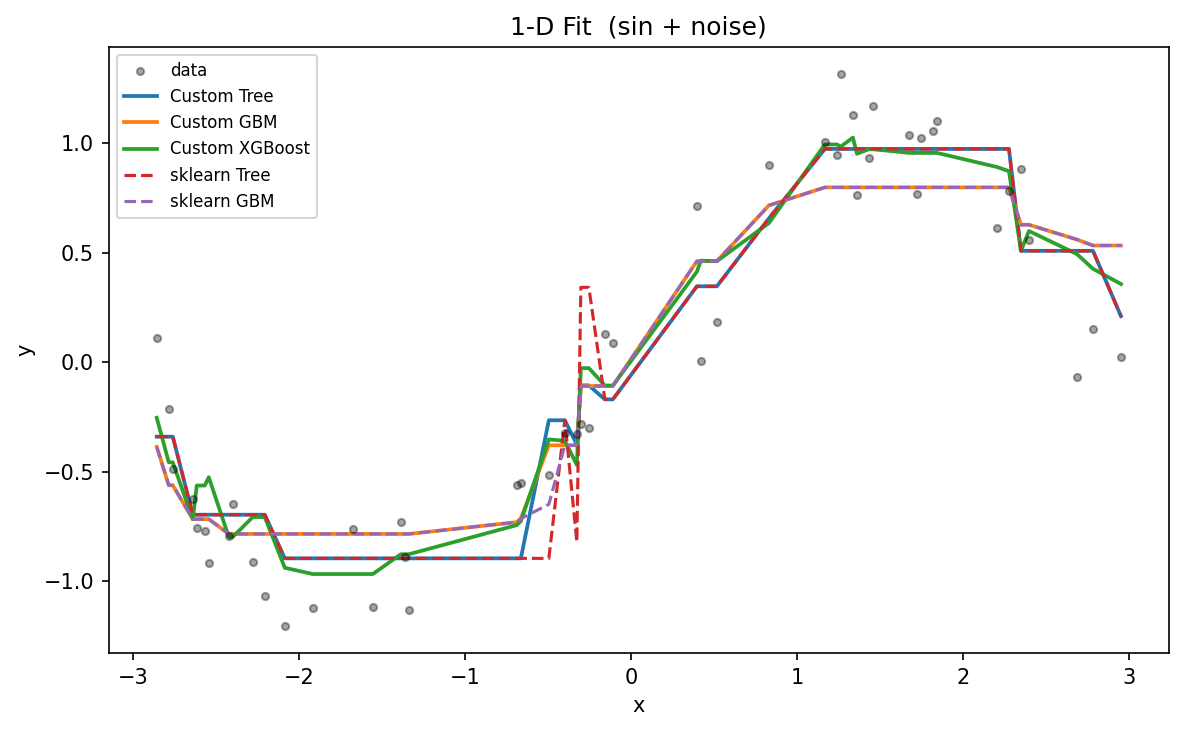
\includegraphics[width=0.43\textwidth]{../plots/1d/fit.png}
  \hfill
  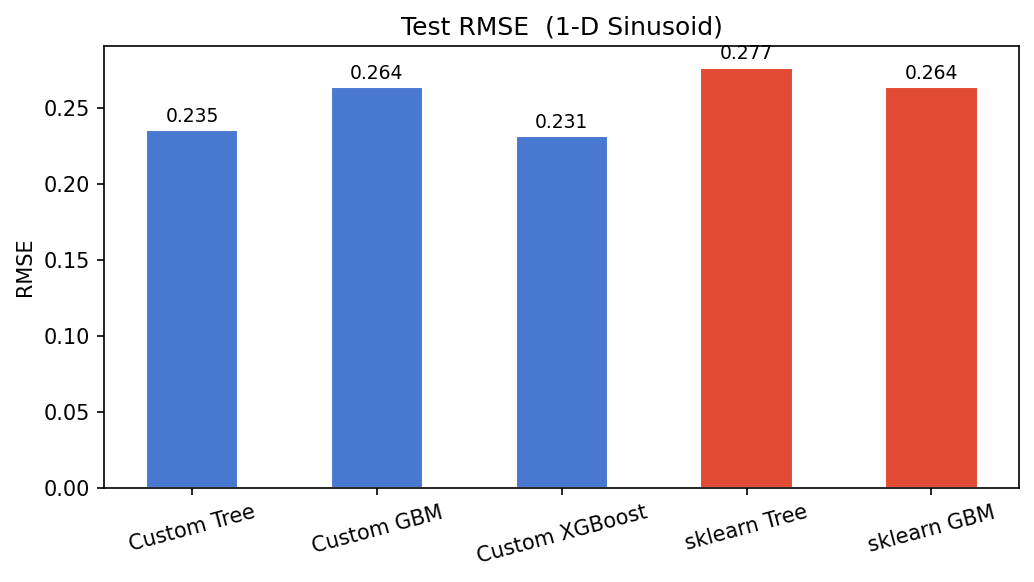
\includegraphics[width=0.43\textwidth]{../plots/1d/rmse.png}
  \caption{1D synthetic dataset: model fit (left) and RMSE
  vs.\ iterations (right).}
\end{figure}

The first data set which we demonstrate in figure 1 the implementations of the
descision tree, gradient boosting model, and XGBoost model is a
synthetic one dimensional dataset of a $\sin$ curve with normally
distributed noise, centered at $\mu = 0$ with $\sigma^2 = 0.5^2$
standard diviation.

Due to the simplicity of this data set, it is easy to see the
behavior of the custom implementations compared to the standard
scikit learn. For instance, the custom GBM and sklearn GBM almsot
entirely overlap, except for the are of very high noise around $x=0$,
where our model seems to have less variance. I'm not exactly sure
what accounts for this difference.

It also demonstrates the relative character of each model, both the
custom and standard desicison trees exhibit higher variance when the
data is noiser while the ensamble methods are slightly more unstable
at regions of the data with low noise, but are much more stable
around the very noisy parts of the data.

\subsection{Natural Datasets}

\subsubsection{California Housing}

The California Housing dataset contains 20,640 census-block records from the
1990 California census. Each sample has eight features: median income,
median house age, average number of rooms and bedrooms, population,
average occupancy, and block latitude and longitude. The target is the
median house value of the block, expressed in units of \$100k. The
full dataset was split 80/20 into train and test sets; because the
custom implementations are considerably slower than sklearn, the
training set was further subsampled to 5,000 rows before fitting.
This experiment is primarily used to evaluate the effect of L2
regularisation: two XGBoost variants are compared, one with
$\lambda = 0$ and one with $\lambda = 1$, alongside the custom GBM
and sklearn's GBM as baselines.

The predicted vs.\ actual hexbin plots show all four models concentrating
density close to the diagonal, with the greatest spread at high values
where the dataset is sparser and the target is capped at 5 (a known
artefact of the original census collection). The residual distributions
are approximately symmetric and centred at zero for every model,
indicating no systematic bias; the main difference between models is the
width of that distribution.

The train vs.\ test RMSE bars reveal a meaningful gap between the custom
implementations and sklearn's GBM, which is expected: the custom models
were trained on a 5,000-row subsample while sklearn saw the full training
set. Within the custom models, XGBoost with $\lambda = 1$ achieves a
slightly lower test RMSE than the unregularised variant, and the train
RMSE gap between the two is smaller than one might expect.

The reason the regularisation effect is modest here connects directly to
the analytical discussion: for MSE loss the Hessian is identically 1 per
sample, so the XGBoost leaf formula $G/(H+\lambda)$ reduces to
$(\sum r_i)/(n + \lambda)$, which is just a slightly shrunk version of
the ordinary mean. The Newton step provides no additional information
beyond what GBM already computes; $\lambda$ acts purely as a shrinkage
factor on leaf values. Consequently GBM and XGBoost are nearly
indistinguishable here, and $\lambda$ plays the same role as a reduced
learning rate would.

\begin{figure}[H]
  \centering
  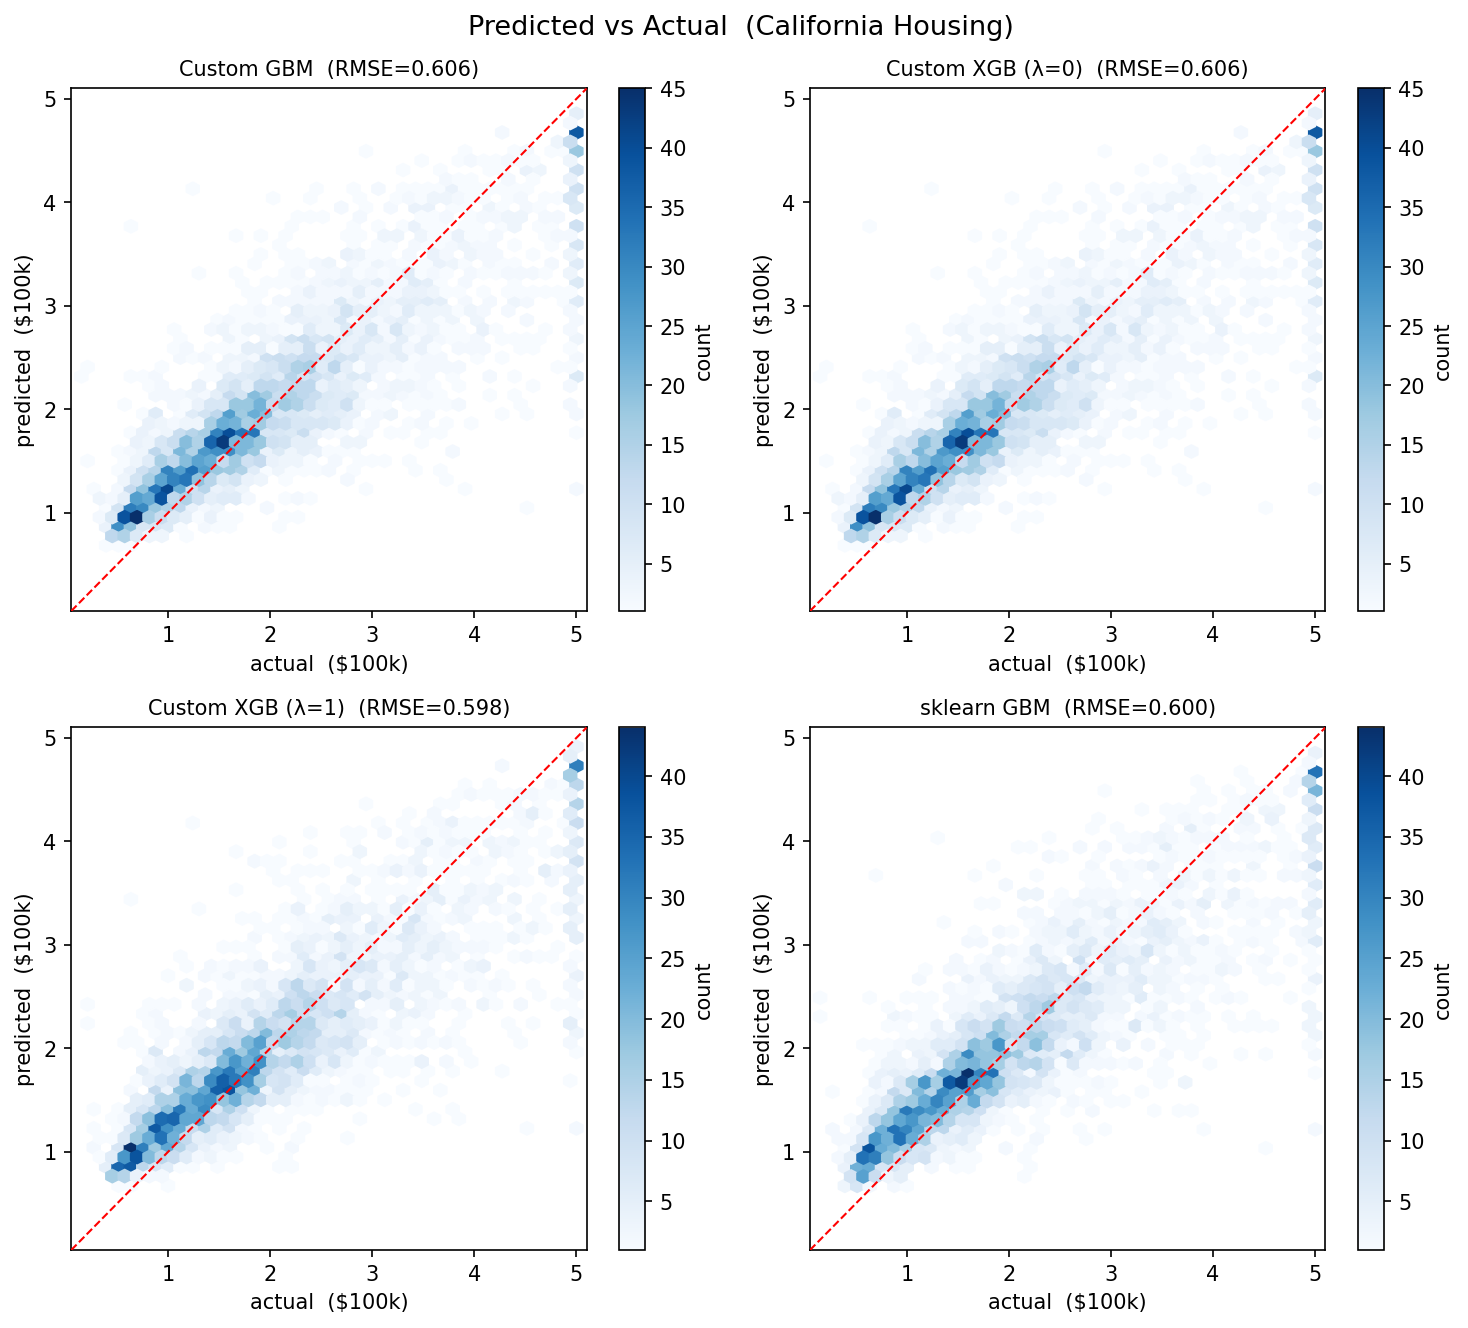
\includegraphics[width=0.43\textwidth]{../plots/california/predicted_vs_actual.png}
  \hfill
  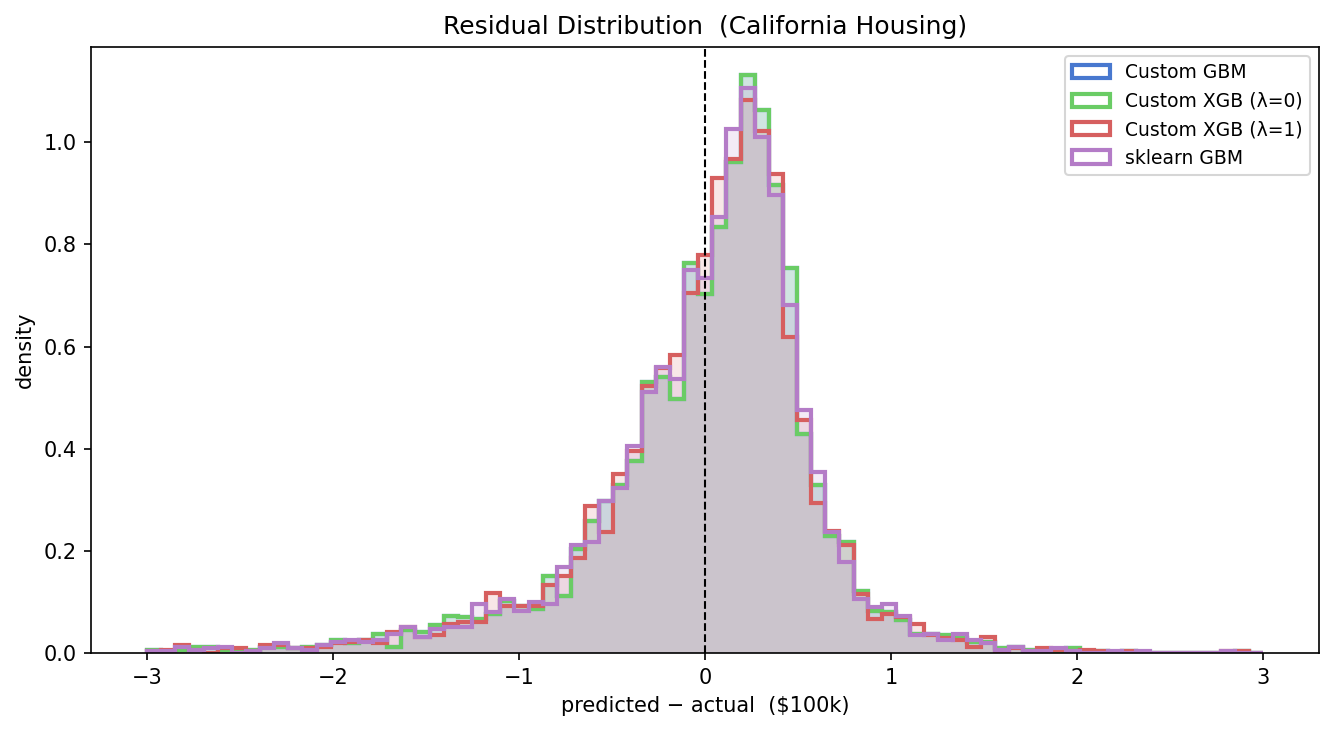
\includegraphics[width=0.43\textwidth]{../plots/california/residuals.png}\\[4pt]
  
\includegraphics[width=0.43\textwidth]{../plots/california/rmse.png}
  \hfill
  
\includegraphics[width=0.43\textwidth]{../plots/california/train_vs_test.png}
  \caption{California housing: predicted vs.\ actual, residuals, RMSE, and
  train/test curves.}
\end{figure}

\subsubsection{Diabetes}

The Diabetes dataset (Efron et al., 2004) consists of 442 patients,
each described by ten baseline features: age, sex, body mass index,
average blood pressure, and six blood serum measurements. All features
are mean-centred and scaled to unit variance. The target is a
quantitative measure of disease progression one year after baseline.
This is a regression task; with only 442 samples it provides a
cleaner comparison of model accuracy without the computational cost
of the larger datasets.

The predicted vs.\ actual scatter shows both ensemble methods tracking
the diagonal reasonably well in the middle of the target range, but
underestimating the highest-progression patients — a common pattern when
the target distribution has a long right tail and training data is sparse
at the extremes.

The more interesting result is that the custom GBM matches or slightly
outperforms XGBoost on this dataset. This is one of the scenarios
discussed in the analysis section where the first-order method can win:
with only 442 samples the Hessian estimates per leaf are noisy, and the
Newton step can overfit to the local curvature of the loss rather than
correcting the residuals in a globally useful direction. For MSE loss the
Hessian is constant so this argument does not apply; however, even the
default MSEHessLoss with $\lambda = 0$ introduces a small amount of
implicit regularisation through the $H$ denominator, which at small leaf
sizes can distort the leaf values relative to the plain mean. The
diabetes dataset sits squarely in the regime where these effects are
non-negligible, making it a useful illustration that XGBoost's advantages
are not unconditional.

\begin{figure}[h]
  \centering
  
\includegraphics[width=0.43\textwidth]{../plots/diabetes/predicted_vs_actual.png}
  \hfill
  
\includegraphics[width=0.43\textwidth]{../plots/diabetes/rmse.png}
  \caption{Diabetes dataset: predicted vs.\ actual and RMSE vs.\ iterations.}
\end{figure}

\subsubsection{Spambase}

The Spambase dataset (UCI) contains 4,601 emails, each labelled as
spam (1) or not spam (0). The 57 features encode the relative
frequency of specific words and characters within the email body, as
well as statistics about runs of consecutive capital letters. This is
a binary classification task; the custom GBM and XGBoost models use
log-loss as the training objective, outputting log-odds which are
converted to class predictions via a sigmoid threshold at 0.5.
Accuracy is reported on an 80/20 train/test split.

Unlike the regression experiments, the log-loss Hessian
$s^i = p^i(1-p^i)$ is non-constant: it is largest when the model is
uncertain ($p \approx 0.5$) and collapses to zero as predictions become
confident. This means XGBoost's Newton step genuinely re-weights
samples — uncertain predictions receive a larger effective learning
signal per iteration than near-certain ones, which is qualitatively
different from the first-order update that treats all residuals equally.

To make the regularisation contrast visible, the trees were allowed an
intentionally excessive maximum depth of 12 over 80 boosting rounds.
At depth 12 a single tree has up to $2^{12} = 4096$ leaves for only
3,680 training samples, so the unregularised model can partition the
training set almost perfectly. The train vs.\ test accuracy plot shows
the consequence: the custom GBM and the weakly-regularised XGBoost
variant accumulate a large train/test gap as the ensemble memorises
idiosyncrasies of the training data. The more strongly regularised
XGBoost variant maintains a noticeably smaller gap, as the $\lambda$
term shrinks each leaf value and the gain threshold implicitly prunes
splits that are not supported by enough gradient mass, preventing the
individual trees from growing to full depth in practice.

This experiment also illustrates the scale-sensitivity of $\lambda$
discussed in the analysis: because log-loss Hessians are bounded above
by 0.25 per sample, a leaf's total $H$ is at most $n_\ell / 4$.
A value of $\lambda = 1$ therefore dominates the denominator for any
leaf with fewer than four samples and has a meaningful shrinkage effect
on leaves with fewer than roughly twenty, which at depth 12 is a large
fraction of all leaves. This is why the regularisation effect is much
more visible here than in the shallower, shorter experiments.

\begin{figure}[h]
  \centering
  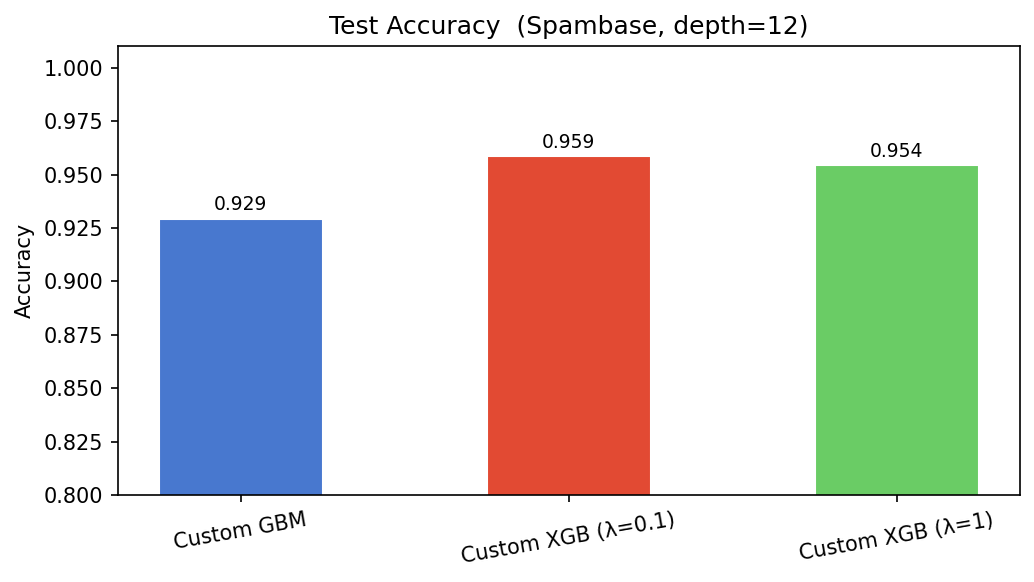
\includegraphics[width=0.43\textwidth]{../plots/spam/accuracy.png}
  \hfill
  
\includegraphics[width=0.43\textwidth]{../plots/spam/train_vs_test.png}
  \caption{Spam classification: accuracy and train/test curves.}
\end{figure}

\subsection{Overfitting}

The overfitting experiment uses a small synthetic regression dataset of
100 samples with 20 features, of which only 5 are informative, generated
by \texttt{sklearn.datasets.make\_regression} with added Gaussian noise.
The target is normalised to zero mean and unit variance. XGBoost is fit
at depth 6 for 30 iterations with four regularisation configurations:
no regularisation ($\lambda = \alpha = \gamma = 0$), L2 only
($\lambda = 3$), L1 only ($\alpha = 1$), and structural regularisation
only ($\gamma = 1$). The 15 non-informative features give the trees many
opportunities to make spurious splits, making this a controlled setting
for isolating the effect of each penalty type. We can see the rough
effects of each type of regularization, $\lambda$ being the most mild
and forgiving to the model, while $\gamma$ prunes the model most
extremly. The L1 and L2 regularizations
that $\lambda$ and $\alpha$ values provide a penalty for large and
extreme leaf values, while $\gamma$ penalizes complex trees.
Arguably, the fact that the XGBoost model exposes all three types of
regularization is what makes it as flexible of a model as it is.

\begin{figure}[h]
  \centering
  
\includegraphics[width=0.55\textwidth]{../plots/overfit/train_vs_test.png}
  \caption{Regularisation comparison: train vs.\ test RMSE for each
  penalty type on the synthetic overfitting dataset.}
\end{figure}

\pagebreak

\section{Conclusions}

We review the requirements for the report:

\textbf{ML family.} This project implements the decision tree and
ensemble family, specifically gradient boosting and the XGBoost variant.

\textbf{Multiple variants.} Three models are implemented: a base
decision tree, a gradient boosting ensemble, and XGBoost; each is a
strict extension of the last.

\textbf{Objective functions and loss functions.} Four loss functions are
provided — MSE, MAE, binary cross-entropy (\texttt{LogLoss}), and its
second-order counterpart (\texttt{LogLossHess}) — along with an
entropy-based node impurity for pure classification trees, and three
regularisation penalties ($\lambda$, $\alpha$, $\gamma$) that are
independently configurable.

\textbf{Regression and classification.} All three models support both
regression and binary classification; the task is selected by swapping
the injected loss object, with no changes to the tree or ensemble code.

\textbf{Mini library.} The implementation is structured as a Python
package under \texttt{models/} with a clean abstract-base-class
hierarchy (\texttt{LossFunction} $\subset$ \texttt{SecondOrderLoss})
that enforces at the type level which losses are compatible with which
models, and experiment scripts kept separately under \texttt{experiments/}.

\textbf{Validation.} The models are benchmarked against scikit-learn's
\texttt{DecisionTreeRegressor} and
\texttt{GradientBoostingRegressor}/\texttt{Classifier}
on five datasets: 1D sinusoid, California Housing, Diabetes, Spambase,
and a synthetic overfitting dataset

\textbf{Correctness checks.} On the 1D sinusoid and diabetes datasets
the custom GBM and sklearn GBM predictions are visually
indistinguishable, and the custom XGBoost matches or approaches sklearn
on all regression tasks, providing an implicit correctness check against
a trusted reference.

\textbf{Visualizations.} Each experiment produces fit curves,
predicted-vs-actual scatter or hexbin plots, residual histograms, and
grouped train/test bar charts; the 1D experiment additionally overlays
all model fits on the raw data for a direct visual comparison.

\textbf{Computational cost.} Computational cost and complexity is
covered in the analysis section.

\textbf{Strengths and weaknesses.} The custom implementation makes every
design decision explicit and the loss function fully user-configurable,
which is useful for understanding the algorithm; in exchange it is slower
than production libraries and does not implement approximate split
finding, column subsampling in the base tree, or GPU support.
Discussion of the specific pros and cons of each model is covered in
the analysis section.

\textbf{Comparison with sklearn.} sklearn's GBM consistently achieves
lower test error on the larger datasets, which is attributable to
training on the full dataset rather than the 5,000-row subsample
required to keep the custom fit time tractable, as well as sklearn's
more efficient internal implementation.

\textbf{Documentation.} The abstract base classes and their methods are
documented with docstrings describing the expected input and output
contract; experiment scripts include inline comments explaining
non-obvious parameter choices and reference the relevant section of the
analysis.

\bibliographystyle{abbrv}
% \bibliography{references}  % need to put bibtex references in references.bib
\end{document}
